\documentclass[twoside]{book}

% Packages required by doxygen
\usepackage{fixltx2e}
\usepackage{calc}
\usepackage{doxygen}
\usepackage[export]{adjustbox} % also loads graphicx
\usepackage{graphicx}
\usepackage[utf8]{inputenc}
\usepackage{makeidx}
\usepackage{multicol}
\usepackage{multirow}
\PassOptionsToPackage{warn}{textcomp}
\usepackage{textcomp}
\usepackage[nointegrals]{wasysym}
\usepackage[table]{xcolor}

% Font selection
\usepackage[T1]{fontenc}
\usepackage[scaled=.90]{helvet}
\usepackage{courier}
\usepackage{amssymb}
\usepackage{sectsty}
\renewcommand{\familydefault}{\sfdefault}
\allsectionsfont{%
  \fontseries{bc}\selectfont%
  \color{darkgray}%
}
\renewcommand{\DoxyLabelFont}{%
  \fontseries{bc}\selectfont%
  \color{darkgray}%
}
\newcommand{\+}{\discretionary{\mbox{\scriptsize$\hookleftarrow$}}{}{}}

% Page & text layout
\usepackage{geometry}
\geometry{%
  a4paper,%
  top=2.5cm,%
  bottom=2.5cm,%
  left=2.5cm,%
  right=2.5cm%
}
\tolerance=750
\hfuzz=15pt
\hbadness=750
\setlength{\emergencystretch}{15pt}
\setlength{\parindent}{0cm}
\setlength{\parskip}{3ex plus 2ex minus 2ex}
\makeatletter
\renewcommand{\paragraph}{%
  \@startsection{paragraph}{4}{0ex}{-1.0ex}{1.0ex}{%
    \normalfont\normalsize\bfseries\SS@parafont%
  }%
}
\renewcommand{\subparagraph}{%
  \@startsection{subparagraph}{5}{0ex}{-1.0ex}{1.0ex}{%
    \normalfont\normalsize\bfseries\SS@subparafont%
  }%
}
\makeatother

% Headers & footers
\usepackage{fancyhdr}
\pagestyle{fancyplain}
\fancyhead[LE]{\fancyplain{}{\bfseries\thepage}}
\fancyhead[CE]{\fancyplain{}{}}
\fancyhead[RE]{\fancyplain{}{\bfseries\leftmark}}
\fancyhead[LO]{\fancyplain{}{\bfseries\rightmark}}
\fancyhead[CO]{\fancyplain{}{}}
\fancyhead[RO]{\fancyplain{}{\bfseries\thepage}}
\fancyfoot[LE]{\fancyplain{}{}}
\fancyfoot[CE]{\fancyplain{}{}}
\fancyfoot[RE]{\fancyplain{}{\bfseries\scriptsize Generated by Doxygen }}
\fancyfoot[LO]{\fancyplain{}{\bfseries\scriptsize Generated by Doxygen }}
\fancyfoot[CO]{\fancyplain{}{}}
\fancyfoot[RO]{\fancyplain{}{}}
\renewcommand{\footrulewidth}{0.4pt}
\renewcommand{\chaptermark}[1]{%
  \markboth{#1}{}%
}
\renewcommand{\sectionmark}[1]{%
  \markright{\thesection\ #1}%
}

% Indices & bibliography
\usepackage{natbib}
\usepackage[titles]{tocloft}
\setcounter{tocdepth}{3}
\setcounter{secnumdepth}{5}
\makeindex

% Hyperlinks (required, but should be loaded last)
\usepackage{ifpdf}
\ifpdf
  \usepackage[pdftex,pagebackref=true]{hyperref}
\else
  \usepackage[ps2pdf,pagebackref=true]{hyperref}
\fi
\hypersetup{%
  colorlinks=true,%
  linkcolor=blue,%
  citecolor=blue,%
  unicode%
}

% Custom commands
\newcommand{\clearemptydoublepage}{%
  \newpage{\pagestyle{empty}\cleardoublepage}%
}

\usepackage{caption}
\captionsetup{labelsep=space,justification=centering,font={bf},singlelinecheck=off,skip=4pt,position=top}

%===== C O N T E N T S =====

\begin{document}

% Titlepage & ToC
\hypersetup{pageanchor=false,
             bookmarksnumbered=true,
             pdfencoding=unicode
            }
\pagenumbering{alph}
\begin{titlepage}
\vspace*{7cm}
\begin{center}%
{\Large Chatterbox \\[1ex]\large 1.\+0 }\\
\vspace*{1cm}
{\large Generated by Doxygen 1.8.13}\\
\end{center}
\end{titlepage}
\clearemptydoublepage
\pagenumbering{roman}
\tableofcontents
\clearemptydoublepage
\pagenumbering{arabic}
\hypersetup{pageanchor=true}

%--- Begin generated contents ---
\chapter{Data Structure Index}
\section{Data Structures}
Here are the data structures with brief descriptions\+:\begin{DoxyCompactList}
\item\contentsline{section}{\hyperlink{structmessage__data__hdr__t}{message\+\_\+data\+\_\+hdr\+\_\+t} \\*Header della parte dati }{\pageref{structmessage__data__hdr__t}}{}
\item\contentsline{section}{\hyperlink{structmessage__data__t}{message\+\_\+data\+\_\+t} \\*Body del messaggio }{\pageref{structmessage__data__t}}{}
\item\contentsline{section}{\hyperlink{structmessage__hdr__t}{message\+\_\+hdr\+\_\+t} \\*Header del messaggio }{\pageref{structmessage__hdr__t}}{}
\item\contentsline{section}{\hyperlink{structmessage__t}{message\+\_\+t} \\*Tipo del messaggio }{\pageref{structmessage__t}}{}
\item\contentsline{section}{\hyperlink{structstatistics}{statistics} }{\pageref{structstatistics}}{}
\end{DoxyCompactList}

\chapter{File Index}
\section{File List}
Here is a list of all documented files with brief descriptions\+:\begin{DoxyCompactList}
\item\contentsline{section}{include/{\bfseries chatty.\+h} }{\pageref{chatty_8h}}{}
\item\contentsline{section}{include/\hyperlink{config_8h}{config.\+h} \\*File contenente alcune define con valori massimi utilizzabili }{\pageref{config_8h}}{}
\item\contentsline{section}{include/\hyperlink{connections_8h}{connections.\+h} \\*Contiene le funzioni che implementano il protocollo tra i clients ed il server }{\pageref{connections_8h}}{}
\item\contentsline{section}{include/{\bfseries log.\+h} }{\pageref{log_8h}}{}
\item\contentsline{section}{include/\hyperlink{message_8h}{message.\+h} \\*Contiene il formato del messaggio }{\pageref{message_8h}}{}
\item\contentsline{section}{include/\hyperlink{ops_8h}{ops.\+h} \\*Contiene i codici delle operazioni di richiesta e risposta }{\pageref{ops_8h}}{}
\item\contentsline{section}{include/{\bfseries server.\+h} }{\pageref{server_8h}}{}
\item\contentsline{section}{include/\hyperlink{signal__handler_8h}{signal\+\_\+handler.\+h} \\*It manages all signals triggered by system }{\pageref{signal__handler_8h}}{}
\item\contentsline{section}{include/{\bfseries stats.\+h} }{\pageref{stats_8h}}{}
\item\contentsline{section}{src/\hyperlink{chatty_8c}{chatty.\+c} \\*File principale del server chatterbox }{\pageref{chatty_8c}}{}
\end{DoxyCompactList}

\chapter{Data Structure Documentation}
\hypertarget{structmessage__data__hdr__t}{}\section{message\+\_\+data\+\_\+hdr\+\_\+t Struct Reference}
\label{structmessage__data__hdr__t}\index{message\+\_\+data\+\_\+hdr\+\_\+t@{message\+\_\+data\+\_\+hdr\+\_\+t}}


header della parte dati  




{\ttfamily \#include $<$message.\+h$>$}

\subsection*{Data Fields}
\begin{DoxyCompactItemize}
\item 
char \hyperlink{structmessage__data__hdr__t_aabb098b2d9fd9305abddad8893b38843}{receiver} \mbox{[}\hyperlink{config_8h_a0c397a708cec89c74029582574516b30}{M\+A\+X\+\_\+\+N\+A\+M\+E\+\_\+\+L\+E\+N\+G\+TH}+1\mbox{]}
\item 
unsigned int \hyperlink{structmessage__data__hdr__t_a77124bd5f7e31e6fffc19f335da0c23f}{len}
\end{DoxyCompactItemize}


\subsection{Detailed Description}
header della parte dati 

\subsection{Field Documentation}
\mbox{\Hypertarget{structmessage__data__hdr__t_a77124bd5f7e31e6fffc19f335da0c23f}\label{structmessage__data__hdr__t_a77124bd5f7e31e6fffc19f335da0c23f}} 
\index{message\+\_\+data\+\_\+hdr\+\_\+t@{message\+\_\+data\+\_\+hdr\+\_\+t}!len@{len}}
\index{len@{len}!message\+\_\+data\+\_\+hdr\+\_\+t@{message\+\_\+data\+\_\+hdr\+\_\+t}}
\subsubsection{\texorpdfstring{len}{len}}
{\footnotesize\ttfamily unsigned int len}

Lunghezza del buffer dati \mbox{\Hypertarget{structmessage__data__hdr__t_aabb098b2d9fd9305abddad8893b38843}\label{structmessage__data__hdr__t_aabb098b2d9fd9305abddad8893b38843}} 
\index{message\+\_\+data\+\_\+hdr\+\_\+t@{message\+\_\+data\+\_\+hdr\+\_\+t}!receiver@{receiver}}
\index{receiver@{receiver}!message\+\_\+data\+\_\+hdr\+\_\+t@{message\+\_\+data\+\_\+hdr\+\_\+t}}
\subsubsection{\texorpdfstring{receiver}{receiver}}
{\footnotesize\ttfamily char receiver\mbox{[}\hyperlink{config_8h_a0c397a708cec89c74029582574516b30}{M\+A\+X\+\_\+\+N\+A\+M\+E\+\_\+\+L\+E\+N\+G\+TH}+1\mbox{]}}

Nickname del ricevente 

The documentation for this struct was generated from the following file\+:\begin{DoxyCompactItemize}
\item 
include/\hyperlink{message_8h}{message.\+h}\end{DoxyCompactItemize}

\hypertarget{structmessage__data__t}{}\section{message\+\_\+data\+\_\+t Struct Reference}
\label{structmessage__data__t}\index{message\+\_\+data\+\_\+t@{message\+\_\+data\+\_\+t}}


body del messaggio  




{\ttfamily \#include $<$message.\+h$>$}



Collaboration diagram for message\+\_\+data\+\_\+t\+:\nopagebreak
\begin{figure}[H]
\begin{center}
\leavevmode
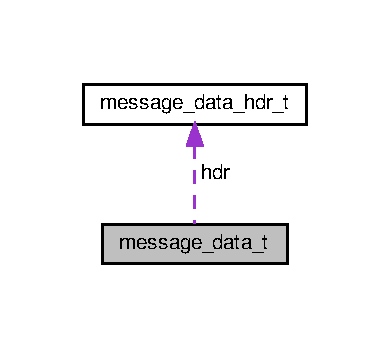
\includegraphics[width=187pt]{structmessage__data__t__coll__graph}
\end{center}
\end{figure}
\subsection*{Data Fields}
\begin{DoxyCompactItemize}
\item 
\hyperlink{structmessage__data__hdr__t}{message\+\_\+data\+\_\+hdr\+\_\+t} \hyperlink{structmessage__data__t_ad76687ebed3a13ddae03410b64f3b134}{hdr}
\item 
char $\ast$ \hyperlink{structmessage__data__t_a1fe855c208bc17a51a4d34fefdb2d5b1}{buf}
\end{DoxyCompactItemize}


\subsection{Detailed Description}
body del messaggio 

\subsection{Field Documentation}
\mbox{\Hypertarget{structmessage__data__t_a1fe855c208bc17a51a4d34fefdb2d5b1}\label{structmessage__data__t_a1fe855c208bc17a51a4d34fefdb2d5b1}} 
\index{message\+\_\+data\+\_\+t@{message\+\_\+data\+\_\+t}!buf@{buf}}
\index{buf@{buf}!message\+\_\+data\+\_\+t@{message\+\_\+data\+\_\+t}}
\subsubsection{\texorpdfstring{buf}{buf}}
{\footnotesize\ttfamily char$\ast$ buf}

Buffer dati \mbox{\Hypertarget{structmessage__data__t_ad76687ebed3a13ddae03410b64f3b134}\label{structmessage__data__t_ad76687ebed3a13ddae03410b64f3b134}} 
\index{message\+\_\+data\+\_\+t@{message\+\_\+data\+\_\+t}!hdr@{hdr}}
\index{hdr@{hdr}!message\+\_\+data\+\_\+t@{message\+\_\+data\+\_\+t}}
\subsubsection{\texorpdfstring{hdr}{hdr}}
{\footnotesize\ttfamily \hyperlink{structmessage__data__hdr__t}{message\+\_\+data\+\_\+hdr\+\_\+t} hdr}

Header della parte dati 

The documentation for this struct was generated from the following file\+:\begin{DoxyCompactItemize}
\item 
include/\hyperlink{message_8h}{message.\+h}\end{DoxyCompactItemize}

\hypertarget{structmessage__hdr__t}{}\section{message\+\_\+hdr\+\_\+t Struct Reference}
\label{structmessage__hdr__t}\index{message\+\_\+hdr\+\_\+t@{message\+\_\+hdr\+\_\+t}}


header del messaggio  




{\ttfamily \#include $<$message.\+h$>$}

\subsection*{Data Fields}
\begin{DoxyCompactItemize}
\item 
\hyperlink{ops_8h_ac6fa1b34da8872e34c2936391332f44c}{op\+\_\+t} \hyperlink{structmessage__hdr__t_a26b2efa792334cce1cd82d1c63754539}{op}
\item 
char \hyperlink{structmessage__hdr__t_a6aa18d82629c912fe68c229936b87c77}{sender} \mbox{[}\hyperlink{config_8h_a0c397a708cec89c74029582574516b30}{M\+A\+X\+\_\+\+N\+A\+M\+E\+\_\+\+L\+E\+N\+G\+TH}+1\mbox{]}
\end{DoxyCompactItemize}


\subsection{Detailed Description}
header del messaggio 

\subsection{Field Documentation}
\mbox{\Hypertarget{structmessage__hdr__t_a26b2efa792334cce1cd82d1c63754539}\label{structmessage__hdr__t_a26b2efa792334cce1cd82d1c63754539}} 
\index{message\+\_\+hdr\+\_\+t@{message\+\_\+hdr\+\_\+t}!op@{op}}
\index{op@{op}!message\+\_\+hdr\+\_\+t@{message\+\_\+hdr\+\_\+t}}
\subsubsection{\texorpdfstring{op}{op}}
{\footnotesize\ttfamily \hyperlink{ops_8h_ac6fa1b34da8872e34c2936391332f44c}{op\+\_\+t} op}

Sipo di connessione richiesta al server \mbox{\Hypertarget{structmessage__hdr__t_a6aa18d82629c912fe68c229936b87c77}\label{structmessage__hdr__t_a6aa18d82629c912fe68c229936b87c77}} 
\index{message\+\_\+hdr\+\_\+t@{message\+\_\+hdr\+\_\+t}!sender@{sender}}
\index{sender@{sender}!message\+\_\+hdr\+\_\+t@{message\+\_\+hdr\+\_\+t}}
\subsubsection{\texorpdfstring{sender}{sender}}
{\footnotesize\ttfamily char sender\mbox{[}\hyperlink{config_8h_a0c397a708cec89c74029582574516b30}{M\+A\+X\+\_\+\+N\+A\+M\+E\+\_\+\+L\+E\+N\+G\+TH}+1\mbox{]}}

Sender nickname del mittente 

The documentation for this struct was generated from the following file\+:\begin{DoxyCompactItemize}
\item 
include/\hyperlink{message_8h}{message.\+h}\end{DoxyCompactItemize}

\hypertarget{structmessage__t}{}\section{message\+\_\+t Struct Reference}
\label{structmessage__t}\index{message\+\_\+t@{message\+\_\+t}}


tipo del messaggio  




{\ttfamily \#include $<$message.\+h$>$}



Collaboration diagram for message\+\_\+t\+:\nopagebreak
\begin{figure}[H]
\begin{center}
\leavevmode
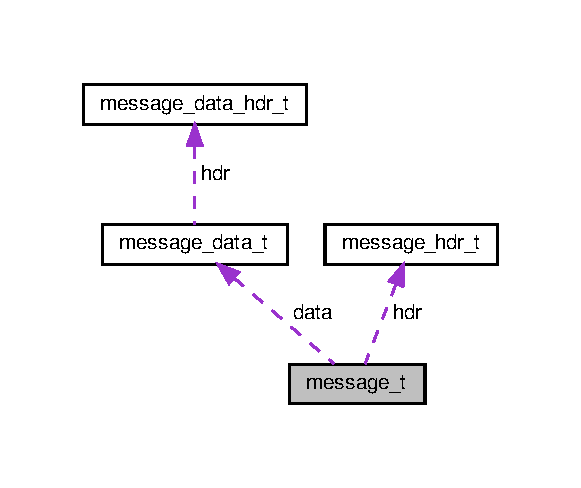
\includegraphics[width=279pt]{structmessage__t__coll__graph}
\end{center}
\end{figure}
\subsection*{Data Fields}
\begin{DoxyCompactItemize}
\item 
\hyperlink{structmessage__hdr__t}{message\+\_\+hdr\+\_\+t} \hyperlink{structmessage__t_ad467c1444d361c52dd802f5609aa9f4c}{hdr}
\item 
\hyperlink{structmessage__data__t}{message\+\_\+data\+\_\+t} \hyperlink{structmessage__t_a4e61df2d2b915250fd442d19a80ca4ca}{data}
\end{DoxyCompactItemize}


\subsection{Detailed Description}
tipo del messaggio 

\subsection{Field Documentation}
\mbox{\Hypertarget{structmessage__t_a4e61df2d2b915250fd442d19a80ca4ca}\label{structmessage__t_a4e61df2d2b915250fd442d19a80ca4ca}} 
\index{message\+\_\+t@{message\+\_\+t}!data@{data}}
\index{data@{data}!message\+\_\+t@{message\+\_\+t}}
\subsubsection{\texorpdfstring{data}{data}}
{\footnotesize\ttfamily \hyperlink{structmessage__data__t}{message\+\_\+data\+\_\+t} data}

Dati del messaggio \mbox{\Hypertarget{structmessage__t_ad467c1444d361c52dd802f5609aa9f4c}\label{structmessage__t_ad467c1444d361c52dd802f5609aa9f4c}} 
\index{message\+\_\+t@{message\+\_\+t}!hdr@{hdr}}
\index{hdr@{hdr}!message\+\_\+t@{message\+\_\+t}}
\subsubsection{\texorpdfstring{hdr}{hdr}}
{\footnotesize\ttfamily \hyperlink{structmessage__hdr__t}{message\+\_\+hdr\+\_\+t} hdr}

Header del messaggio 

The documentation for this struct was generated from the following file\+:\begin{DoxyCompactItemize}
\item 
include/\hyperlink{message_8h}{message.\+h}\end{DoxyCompactItemize}

\hypertarget{structstatistics}{}\section{statistics Struct Reference}
\label{structstatistics}\index{statistics@{statistics}}


{\ttfamily \#include $<$stats.\+h$>$}

\subsection*{Data Fields}
\begin{DoxyCompactItemize}
\item 
unsigned long \hyperlink{structstatistics_adacd907234b18252c5e1ec947deca41f}{nusers}
\item 
unsigned long \hyperlink{structstatistics_aff99cf9b6aa2d22f48f543a906603ae7}{nonline}
\item 
unsigned long \hyperlink{structstatistics_a08e845e3d8ec6f288e20a4693ff09123}{ndelivered}
\item 
unsigned long \hyperlink{structstatistics_a544cca2dcba9741ea008e54ab3b4eef8}{nnotdelivered}
\item 
unsigned long \hyperlink{structstatistics_a0b799597236f59771d2df823cc295de1}{nfiledelivered}
\item 
unsigned long \hyperlink{structstatistics_a3f46d11b2e9a9b2cf0294f5f55fe3d32}{nfilenotdelivered}
\item 
unsigned long \hyperlink{structstatistics_a6b8853d9bf908c15a1c6444ac8e62c20}{nerrors}
\end{DoxyCompactItemize}


\subsection{Detailed Description}
Statistics structure. 

\subsection{Field Documentation}
\mbox{\Hypertarget{structstatistics_a08e845e3d8ec6f288e20a4693ff09123}\label{structstatistics_a08e845e3d8ec6f288e20a4693ff09123}} 
\index{statistics@{statistics}!ndelivered@{ndelivered}}
\index{ndelivered@{ndelivered}!statistics@{statistics}}
\subsubsection{\texorpdfstring{ndelivered}{ndelivered}}
{\footnotesize\ttfamily unsigned long ndelivered}

Number of delivered messages \mbox{\Hypertarget{structstatistics_a6b8853d9bf908c15a1c6444ac8e62c20}\label{structstatistics_a6b8853d9bf908c15a1c6444ac8e62c20}} 
\index{statistics@{statistics}!nerrors@{nerrors}}
\index{nerrors@{nerrors}!statistics@{statistics}}
\subsubsection{\texorpdfstring{nerrors}{nerrors}}
{\footnotesize\ttfamily unsigned long nerrors}

Number of errors \mbox{\Hypertarget{structstatistics_a0b799597236f59771d2df823cc295de1}\label{structstatistics_a0b799597236f59771d2df823cc295de1}} 
\index{statistics@{statistics}!nfiledelivered@{nfiledelivered}}
\index{nfiledelivered@{nfiledelivered}!statistics@{statistics}}
\subsubsection{\texorpdfstring{nfiledelivered}{nfiledelivered}}
{\footnotesize\ttfamily unsigned long nfiledelivered}

Number of file delivered \mbox{\Hypertarget{structstatistics_a3f46d11b2e9a9b2cf0294f5f55fe3d32}\label{structstatistics_a3f46d11b2e9a9b2cf0294f5f55fe3d32}} 
\index{statistics@{statistics}!nfilenotdelivered@{nfilenotdelivered}}
\index{nfilenotdelivered@{nfilenotdelivered}!statistics@{statistics}}
\subsubsection{\texorpdfstring{nfilenotdelivered}{nfilenotdelivered}}
{\footnotesize\ttfamily unsigned long nfilenotdelivered}

Number of file not delivered \mbox{\Hypertarget{structstatistics_a544cca2dcba9741ea008e54ab3b4eef8}\label{structstatistics_a544cca2dcba9741ea008e54ab3b4eef8}} 
\index{statistics@{statistics}!nnotdelivered@{nnotdelivered}}
\index{nnotdelivered@{nnotdelivered}!statistics@{statistics}}
\subsubsection{\texorpdfstring{nnotdelivered}{nnotdelivered}}
{\footnotesize\ttfamily unsigned long nnotdelivered}

Number of not delivered messages \mbox{\Hypertarget{structstatistics_aff99cf9b6aa2d22f48f543a906603ae7}\label{structstatistics_aff99cf9b6aa2d22f48f543a906603ae7}} 
\index{statistics@{statistics}!nonline@{nonline}}
\index{nonline@{nonline}!statistics@{statistics}}
\subsubsection{\texorpdfstring{nonline}{nonline}}
{\footnotesize\ttfamily unsigned long nonline}

Online users \mbox{\Hypertarget{structstatistics_adacd907234b18252c5e1ec947deca41f}\label{structstatistics_adacd907234b18252c5e1ec947deca41f}} 
\index{statistics@{statistics}!nusers@{nusers}}
\index{nusers@{nusers}!statistics@{statistics}}
\subsubsection{\texorpdfstring{nusers}{nusers}}
{\footnotesize\ttfamily unsigned long nusers}

Registered users 

The documentation for this struct was generated from the following file\+:\begin{DoxyCompactItemize}
\item 
include/stats.\+h\end{DoxyCompactItemize}

\chapter{File Documentation}
\hypertarget{config_8h}{}\section{include/config.h File Reference}
\label{config_8h}\index{include/config.\+h@{include/config.\+h}}


File contenente alcune define con valori massimi utilizzabili.  


This graph shows which files directly or indirectly include this file\+:\nopagebreak
\begin{figure}[H]
\begin{center}
\leavevmode
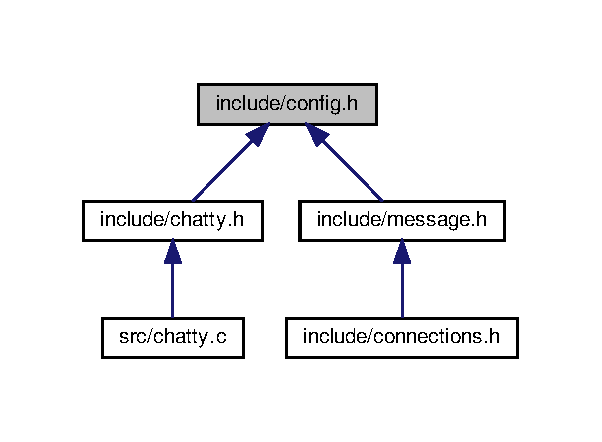
\includegraphics[width=289pt]{config_8h__dep__incl}
\end{center}
\end{figure}
\subsection*{Macros}
\begin{DoxyCompactItemize}
\item 
\#define \hyperlink{config_8h_a0c397a708cec89c74029582574516b30}{M\+A\+X\+\_\+\+N\+A\+M\+E\+\_\+\+L\+E\+N\+G\+TH}~32
\item 
\#define \hyperlink{config_8h_ae4e5f1b7666fdf5484d616f09aed4fec}{C\+O\+N\+F\+I\+G\+\_\+\+R\+E\+Q\+U\+I\+R\+E\+D\+\_\+\+P\+A\+R\+A\+M\+S\+\_\+\+S\+I\+ZE}~8
\item 
\#define \hyperlink{config_8h_a2bdac4fecfc297552c3f51f9aa5bcac8}{C\+O\+N\+F\+\_\+\+S\+T\+R\+I\+N\+G\+\_\+T}~0
\item 
\#define \hyperlink{config_8h_afc03bcd0280286fa764eca8d95fc2b12}{C\+O\+N\+F\+\_\+\+I\+N\+T\+\_\+T}~1
\end{DoxyCompactItemize}
\subsection*{Typedefs}
\begin{DoxyCompactItemize}
\item 
typedef int \hyperlink{config_8h_a7aced504ae5e6032aeb8dd0a72fcb5bc}{make\+\_\+iso\+\_\+compilers\+\_\+happy}
\end{DoxyCompactItemize}


\subsection{Detailed Description}
File contenente alcune define con valori massimi utilizzabili. 



\subsection{Macro Definition Documentation}
\mbox{\Hypertarget{config_8h_afc03bcd0280286fa764eca8d95fc2b12}\label{config_8h_afc03bcd0280286fa764eca8d95fc2b12}} 
\index{config.\+h@{config.\+h}!C\+O\+N\+F\+\_\+\+I\+N\+T\+\_\+T@{C\+O\+N\+F\+\_\+\+I\+N\+T\+\_\+T}}
\index{C\+O\+N\+F\+\_\+\+I\+N\+T\+\_\+T@{C\+O\+N\+F\+\_\+\+I\+N\+T\+\_\+T}!config.\+h@{config.\+h}}
\subsubsection{\texorpdfstring{C\+O\+N\+F\+\_\+\+I\+N\+T\+\_\+T}{CONF\_INT\_T}}
{\footnotesize\ttfamily \#define C\+O\+N\+F\+\_\+\+I\+N\+T\+\_\+T~1}

Represents the integer type of configuration parameter \mbox{\Hypertarget{config_8h_a2bdac4fecfc297552c3f51f9aa5bcac8}\label{config_8h_a2bdac4fecfc297552c3f51f9aa5bcac8}} 
\index{config.\+h@{config.\+h}!C\+O\+N\+F\+\_\+\+S\+T\+R\+I\+N\+G\+\_\+T@{C\+O\+N\+F\+\_\+\+S\+T\+R\+I\+N\+G\+\_\+T}}
\index{C\+O\+N\+F\+\_\+\+S\+T\+R\+I\+N\+G\+\_\+T@{C\+O\+N\+F\+\_\+\+S\+T\+R\+I\+N\+G\+\_\+T}!config.\+h@{config.\+h}}
\subsubsection{\texorpdfstring{C\+O\+N\+F\+\_\+\+S\+T\+R\+I\+N\+G\+\_\+T}{CONF\_STRING\_T}}
{\footnotesize\ttfamily \#define C\+O\+N\+F\+\_\+\+S\+T\+R\+I\+N\+G\+\_\+T~0}

Represents the string type of configuration parameter \mbox{\Hypertarget{config_8h_ae4e5f1b7666fdf5484d616f09aed4fec}\label{config_8h_ae4e5f1b7666fdf5484d616f09aed4fec}} 
\index{config.\+h@{config.\+h}!C\+O\+N\+F\+I\+G\+\_\+\+R\+E\+Q\+U\+I\+R\+E\+D\+\_\+\+P\+A\+R\+A\+M\+S\+\_\+\+S\+I\+ZE@{C\+O\+N\+F\+I\+G\+\_\+\+R\+E\+Q\+U\+I\+R\+E\+D\+\_\+\+P\+A\+R\+A\+M\+S\+\_\+\+S\+I\+ZE}}
\index{C\+O\+N\+F\+I\+G\+\_\+\+R\+E\+Q\+U\+I\+R\+E\+D\+\_\+\+P\+A\+R\+A\+M\+S\+\_\+\+S\+I\+ZE@{C\+O\+N\+F\+I\+G\+\_\+\+R\+E\+Q\+U\+I\+R\+E\+D\+\_\+\+P\+A\+R\+A\+M\+S\+\_\+\+S\+I\+ZE}!config.\+h@{config.\+h}}
\subsubsection{\texorpdfstring{C\+O\+N\+F\+I\+G\+\_\+\+R\+E\+Q\+U\+I\+R\+E\+D\+\_\+\+P\+A\+R\+A\+M\+S\+\_\+\+S\+I\+ZE}{CONFIG\_REQUIRED\_PARAMS\_SIZE}}
{\footnotesize\ttfamily \#define C\+O\+N\+F\+I\+G\+\_\+\+R\+E\+Q\+U\+I\+R\+E\+D\+\_\+\+P\+A\+R\+A\+M\+S\+\_\+\+S\+I\+ZE~8}

Size of array that contains required configuration parameters \mbox{\Hypertarget{config_8h_a0c397a708cec89c74029582574516b30}\label{config_8h_a0c397a708cec89c74029582574516b30}} 
\index{config.\+h@{config.\+h}!M\+A\+X\+\_\+\+N\+A\+M\+E\+\_\+\+L\+E\+N\+G\+TH@{M\+A\+X\+\_\+\+N\+A\+M\+E\+\_\+\+L\+E\+N\+G\+TH}}
\index{M\+A\+X\+\_\+\+N\+A\+M\+E\+\_\+\+L\+E\+N\+G\+TH@{M\+A\+X\+\_\+\+N\+A\+M\+E\+\_\+\+L\+E\+N\+G\+TH}!config.\+h@{config.\+h}}
\subsubsection{\texorpdfstring{M\+A\+X\+\_\+\+N\+A\+M\+E\+\_\+\+L\+E\+N\+G\+TH}{MAX\_NAME\_LENGTH}}
{\footnotesize\ttfamily \#define M\+A\+X\+\_\+\+N\+A\+M\+E\+\_\+\+L\+E\+N\+G\+TH~32}

Max length of user name 

\subsection{Typedef Documentation}
\mbox{\Hypertarget{config_8h_a7aced504ae5e6032aeb8dd0a72fcb5bc}\label{config_8h_a7aced504ae5e6032aeb8dd0a72fcb5bc}} 
\index{config.\+h@{config.\+h}!make\+\_\+iso\+\_\+compilers\+\_\+happy@{make\+\_\+iso\+\_\+compilers\+\_\+happy}}
\index{make\+\_\+iso\+\_\+compilers\+\_\+happy@{make\+\_\+iso\+\_\+compilers\+\_\+happy}!config.\+h@{config.\+h}}
\subsubsection{\texorpdfstring{make\+\_\+iso\+\_\+compilers\+\_\+happy}{make\_iso\_compilers\_happy}}
{\footnotesize\ttfamily typedef int \hyperlink{config_8h_a7aced504ae5e6032aeb8dd0a72fcb5bc}{make\+\_\+iso\+\_\+compilers\+\_\+happy}}

to avoid warnings like \char`\"{}\+I\+S\+O C forbids an empty translation unit\char`\"{} 
\hypertarget{connections_8h}{}\section{include/connections.h File Reference}
\label{connections_8h}\index{include/connections.\+h@{include/connections.\+h}}


Contiene le funzioni che implementano il protocollo tra i clients ed il server.  


{\ttfamily \#include $<$message.\+h$>$}\newline
Include dependency graph for connections.\+h\+:\nopagebreak
\begin{figure}[H]
\begin{center}
\leavevmode
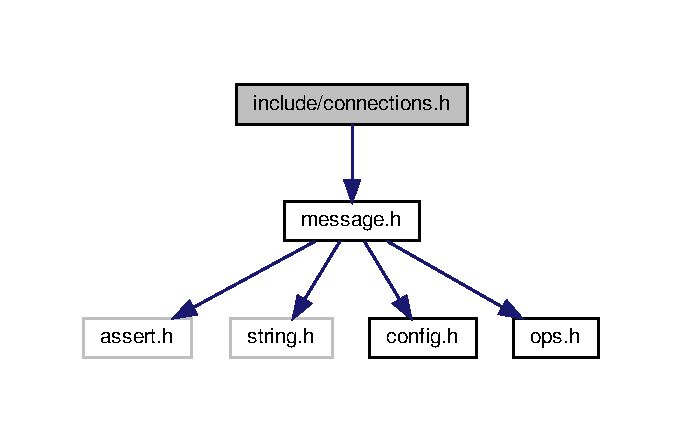
\includegraphics[width=328pt]{connections_8h__incl}
\end{center}
\end{figure}
\subsection*{Macros}
\begin{DoxyCompactItemize}
\item 
\#define \hyperlink{connections_8h_aecf13b8dc783db2202ca5c34fe117fc3}{M\+A\+X\+\_\+\+R\+E\+T\+R\+I\+ES}~10
\item 
\#define \hyperlink{connections_8h_a763a071b50fb9cf7997861d0f5266387}{M\+A\+X\+\_\+\+S\+L\+E\+E\+P\+I\+NG}~3
\item 
\#define \hyperlink{connections_8h_a7baab2aa5bf8eb14b6128e0f16634837}{U\+N\+I\+X\+\_\+\+P\+A\+T\+H\+\_\+\+M\+AX}~64
\end{DoxyCompactItemize}
\subsection*{Functions}
\begin{DoxyCompactItemize}
\item 
int \hyperlink{connections_8h_a93ad31c416b2e2055827e5f684e89daf}{open\+Connection} (char $\ast$path, unsigned int ntimes, unsigned int secs)
\begin{DoxyCompactList}\small\item\em Apre una connessione A\+F\+\_\+\+U\+N\+IX verso il server. \end{DoxyCompactList}\item 
int \hyperlink{connections_8h_a2a15cc3debfd6700ea0f40a198c55c85}{read\+Header} (long connfd, \hyperlink{structmessage__hdr__t}{message\+\_\+hdr\+\_\+t} $\ast$hdr)
\begin{DoxyCompactList}\small\item\em Legge l\textquotesingle{}header del messaggio. \end{DoxyCompactList}\item 
int \hyperlink{connections_8h_acf5cb8379636265d11a008d6aa94dc30}{read\+Data} (long fd, \hyperlink{structmessage__data__t}{message\+\_\+data\+\_\+t} $\ast$data)
\begin{DoxyCompactList}\small\item\em Legge il body del messaggio. \end{DoxyCompactList}\item 
int \hyperlink{connections_8h_a2fc6b845d44636fb241a848e58c83420}{read\+Msg} (long fd, \hyperlink{structmessage__t}{message\+\_\+t} $\ast$msg)
\begin{DoxyCompactList}\small\item\em Legge l\textquotesingle{}intero messaggio. \end{DoxyCompactList}\item 
int \hyperlink{connections_8h_a3c23eb25de2ae8b5216eb6dd847521c0}{send\+Request} (long fd, \hyperlink{structmessage__t}{message\+\_\+t} $\ast$msg)
\begin{DoxyCompactList}\small\item\em Invia un messaggio di richiesta al server. \end{DoxyCompactList}\item 
int \hyperlink{connections_8h_a7812cf59eeeaa63ce7d7b9ce93125462}{send\+Data} (long fd, \hyperlink{structmessage__data__t}{message\+\_\+data\+\_\+t} $\ast$msg)
\begin{DoxyCompactList}\small\item\em Invia il body del messaggio al server. \end{DoxyCompactList}\end{DoxyCompactItemize}


\subsection{Detailed Description}
Contiene le funzioni che implementano il protocollo tra i clients ed il server. 



\subsection{Macro Definition Documentation}
\mbox{\Hypertarget{connections_8h_aecf13b8dc783db2202ca5c34fe117fc3}\label{connections_8h_aecf13b8dc783db2202ca5c34fe117fc3}} 
\index{connections.\+h@{connections.\+h}!M\+A\+X\+\_\+\+R\+E\+T\+R\+I\+ES@{M\+A\+X\+\_\+\+R\+E\+T\+R\+I\+ES}}
\index{M\+A\+X\+\_\+\+R\+E\+T\+R\+I\+ES@{M\+A\+X\+\_\+\+R\+E\+T\+R\+I\+ES}!connections.\+h@{connections.\+h}}
\subsubsection{\texorpdfstring{M\+A\+X\+\_\+\+R\+E\+T\+R\+I\+ES}{MAX\_RETRIES}}
{\footnotesize\ttfamily \#define M\+A\+X\+\_\+\+R\+E\+T\+R\+I\+ES~10}

How many time retry to send message. \mbox{\Hypertarget{connections_8h_a763a071b50fb9cf7997861d0f5266387}\label{connections_8h_a763a071b50fb9cf7997861d0f5266387}} 
\index{connections.\+h@{connections.\+h}!M\+A\+X\+\_\+\+S\+L\+E\+E\+P\+I\+NG@{M\+A\+X\+\_\+\+S\+L\+E\+E\+P\+I\+NG}}
\index{M\+A\+X\+\_\+\+S\+L\+E\+E\+P\+I\+NG@{M\+A\+X\+\_\+\+S\+L\+E\+E\+P\+I\+NG}!connections.\+h@{connections.\+h}}
\subsubsection{\texorpdfstring{M\+A\+X\+\_\+\+S\+L\+E\+E\+P\+I\+NG}{MAX\_SLEEPING}}
{\footnotesize\ttfamily \#define M\+A\+X\+\_\+\+S\+L\+E\+E\+P\+I\+NG~3}

How many time a server can sleep. \mbox{\Hypertarget{connections_8h_a7baab2aa5bf8eb14b6128e0f16634837}\label{connections_8h_a7baab2aa5bf8eb14b6128e0f16634837}} 
\index{connections.\+h@{connections.\+h}!U\+N\+I\+X\+\_\+\+P\+A\+T\+H\+\_\+\+M\+AX@{U\+N\+I\+X\+\_\+\+P\+A\+T\+H\+\_\+\+M\+AX}}
\index{U\+N\+I\+X\+\_\+\+P\+A\+T\+H\+\_\+\+M\+AX@{U\+N\+I\+X\+\_\+\+P\+A\+T\+H\+\_\+\+M\+AX}!connections.\+h@{connections.\+h}}
\subsubsection{\texorpdfstring{U\+N\+I\+X\+\_\+\+P\+A\+T\+H\+\_\+\+M\+AX}{UNIX\_PATH\_MAX}}
{\footnotesize\ttfamily \#define U\+N\+I\+X\+\_\+\+P\+A\+T\+H\+\_\+\+M\+AX~64}

U\+N\+IX path max definition. 

\subsection{Function Documentation}
\mbox{\Hypertarget{connections_8h_a93ad31c416b2e2055827e5f684e89daf}\label{connections_8h_a93ad31c416b2e2055827e5f684e89daf}} 
\index{connections.\+h@{connections.\+h}!open\+Connection@{open\+Connection}}
\index{open\+Connection@{open\+Connection}!connections.\+h@{connections.\+h}}
\subsubsection{\texorpdfstring{open\+Connection()}{openConnection()}}
{\footnotesize\ttfamily int open\+Connection (\begin{DoxyParamCaption}\item[{char $\ast$}]{path,  }\item[{unsigned int}]{ntimes,  }\item[{unsigned int}]{secs }\end{DoxyParamCaption})}



Apre una connessione A\+F\+\_\+\+U\+N\+IX verso il server. 


\begin{DoxyParams}{Parameters}
{\em path} & Path del socket A\+F\+\_\+\+U\+N\+IX \\
\hline
{\em ntimes} & numero massimo di tentativi di retry \\
\hline
{\em secs} & tempo di attesa tra due retry consecutive\\
\hline
\end{DoxyParams}
\begin{DoxyReturn}{Returns}
il descrittore associato alla connessione in caso di successo -\/1 in caso di errore 
\end{DoxyReturn}
\mbox{\Hypertarget{connections_8h_acf5cb8379636265d11a008d6aa94dc30}\label{connections_8h_acf5cb8379636265d11a008d6aa94dc30}} 
\index{connections.\+h@{connections.\+h}!read\+Data@{read\+Data}}
\index{read\+Data@{read\+Data}!connections.\+h@{connections.\+h}}
\subsubsection{\texorpdfstring{read\+Data()}{readData()}}
{\footnotesize\ttfamily int read\+Data (\begin{DoxyParamCaption}\item[{long}]{fd,  }\item[{\hyperlink{structmessage__data__t}{message\+\_\+data\+\_\+t} $\ast$}]{data }\end{DoxyParamCaption})}



Legge il body del messaggio. 


\begin{DoxyParams}{Parameters}
{\em fd} & descrittore della connessione \\
\hline
{\em data} & puntatore al body del messaggio\\
\hline
\end{DoxyParams}
\begin{DoxyReturn}{Returns}
$<$=0 se c\textquotesingle{}e\textquotesingle{} stato un errore (se $<$0 errno deve essere settato, se == 0 connessione chiusa) 
\end{DoxyReturn}
\mbox{\Hypertarget{connections_8h_a2a15cc3debfd6700ea0f40a198c55c85}\label{connections_8h_a2a15cc3debfd6700ea0f40a198c55c85}} 
\index{connections.\+h@{connections.\+h}!read\+Header@{read\+Header}}
\index{read\+Header@{read\+Header}!connections.\+h@{connections.\+h}}
\subsubsection{\texorpdfstring{read\+Header()}{readHeader()}}
{\footnotesize\ttfamily int read\+Header (\begin{DoxyParamCaption}\item[{long}]{connfd,  }\item[{\hyperlink{structmessage__hdr__t}{message\+\_\+hdr\+\_\+t} $\ast$}]{hdr }\end{DoxyParamCaption})}



Legge l\textquotesingle{}header del messaggio. 


\begin{DoxyParams}{Parameters}
{\em connfd} & descrittore della connessione \\
\hline
{\em hdr} & puntatore all\textquotesingle{}header del messaggio da ricevere\\
\hline
\end{DoxyParams}
\begin{DoxyReturn}{Returns}
$<$=0 se c\textquotesingle{}e\textquotesingle{} stato un errore (se $<$0 errno deve essere settato, se == 0 connessione chiusa) 
\end{DoxyReturn}
\mbox{\Hypertarget{connections_8h_a2fc6b845d44636fb241a848e58c83420}\label{connections_8h_a2fc6b845d44636fb241a848e58c83420}} 
\index{connections.\+h@{connections.\+h}!read\+Msg@{read\+Msg}}
\index{read\+Msg@{read\+Msg}!connections.\+h@{connections.\+h}}
\subsubsection{\texorpdfstring{read\+Msg()}{readMsg()}}
{\footnotesize\ttfamily int read\+Msg (\begin{DoxyParamCaption}\item[{long}]{fd,  }\item[{\hyperlink{structmessage__t}{message\+\_\+t} $\ast$}]{msg }\end{DoxyParamCaption})}



Legge l\textquotesingle{}intero messaggio. 


\begin{DoxyParams}{Parameters}
{\em fd} & descrittore della connessione \\
\hline
{\em msg} & puntatore al messaggio\\
\hline
\end{DoxyParams}
\begin{DoxyReturn}{Returns}
$<$=0 se c\textquotesingle{}e\textquotesingle{} stato un errore (se $<$0 errno deve essere settato, se == 0 connessione chiusa) 
\end{DoxyReturn}
\mbox{\Hypertarget{connections_8h_a7812cf59eeeaa63ce7d7b9ce93125462}\label{connections_8h_a7812cf59eeeaa63ce7d7b9ce93125462}} 
\index{connections.\+h@{connections.\+h}!send\+Data@{send\+Data}}
\index{send\+Data@{send\+Data}!connections.\+h@{connections.\+h}}
\subsubsection{\texorpdfstring{send\+Data()}{sendData()}}
{\footnotesize\ttfamily int send\+Data (\begin{DoxyParamCaption}\item[{long}]{fd,  }\item[{\hyperlink{structmessage__data__t}{message\+\_\+data\+\_\+t} $\ast$}]{msg }\end{DoxyParamCaption})}



Invia il body del messaggio al server. 


\begin{DoxyParams}{Parameters}
{\em fd} & descrittore della connessione \\
\hline
{\em msg} & puntatore al messaggio da inviare\\
\hline
\end{DoxyParams}
\begin{DoxyReturn}{Returns}
$<$=0 se c\textquotesingle{}e\textquotesingle{} stato un errore 
\end{DoxyReturn}
\mbox{\Hypertarget{connections_8h_a3c23eb25de2ae8b5216eb6dd847521c0}\label{connections_8h_a3c23eb25de2ae8b5216eb6dd847521c0}} 
\index{connections.\+h@{connections.\+h}!send\+Request@{send\+Request}}
\index{send\+Request@{send\+Request}!connections.\+h@{connections.\+h}}
\subsubsection{\texorpdfstring{send\+Request()}{sendRequest()}}
{\footnotesize\ttfamily int send\+Request (\begin{DoxyParamCaption}\item[{long}]{fd,  }\item[{\hyperlink{structmessage__t}{message\+\_\+t} $\ast$}]{msg }\end{DoxyParamCaption})}



Invia un messaggio di richiesta al server. 


\begin{DoxyParams}{Parameters}
{\em fd} & descrittore della connessione \\
\hline
{\em msg} & puntatore al messaggio da inviare\\
\hline
\end{DoxyParams}
\begin{DoxyReturn}{Returns}
$<$=0 se c\textquotesingle{}e\textquotesingle{} stato un errore 
\end{DoxyReturn}

\hypertarget{message_8h}{}\section{include/message.h File Reference}
\label{message_8h}\index{include/message.\+h@{include/message.\+h}}


Contiene il formato del messaggio.  


{\ttfamily \#include $<$assert.\+h$>$}\newline
{\ttfamily \#include $<$string.\+h$>$}\newline
{\ttfamily \#include $<$config.\+h$>$}\newline
{\ttfamily \#include \char`\"{}ops.\+h\char`\"{}}\newline
Include dependency graph for message.\+h\+:\nopagebreak
\begin{figure}[H]
\begin{center}
\leavevmode
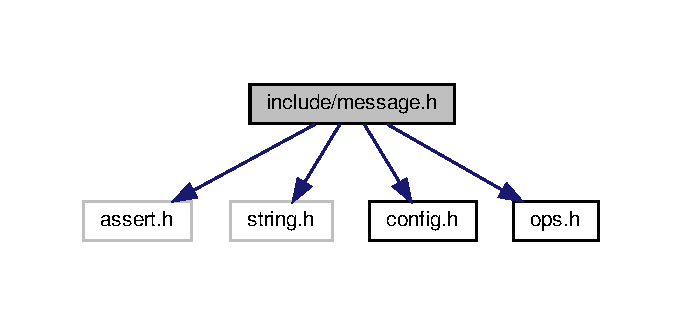
\includegraphics[width=328pt]{message_8h__incl}
\end{center}
\end{figure}
This graph shows which files directly or indirectly include this file\+:\nopagebreak
\begin{figure}[H]
\begin{center}
\leavevmode
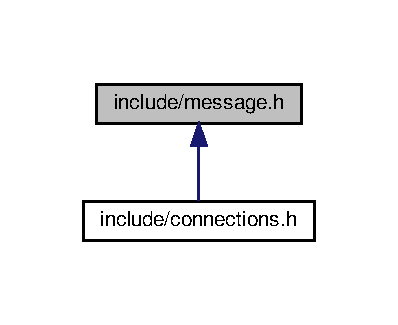
\includegraphics[width=191pt]{message_8h__dep__incl}
\end{center}
\end{figure}
\subsection*{Data Structures}
\begin{DoxyCompactItemize}
\item 
struct \hyperlink{structmessage__hdr__t}{message\+\_\+hdr\+\_\+t}
\begin{DoxyCompactList}\small\item\em header del messaggio \end{DoxyCompactList}\item 
struct \hyperlink{structmessage__data__hdr__t}{message\+\_\+data\+\_\+hdr\+\_\+t}
\begin{DoxyCompactList}\small\item\em header della parte dati \end{DoxyCompactList}\item 
struct \hyperlink{structmessage__data__t}{message\+\_\+data\+\_\+t}
\begin{DoxyCompactList}\small\item\em body del messaggio \end{DoxyCompactList}\item 
struct \hyperlink{structmessage__t}{message\+\_\+t}
\begin{DoxyCompactList}\small\item\em tipo del messaggio \end{DoxyCompactList}\end{DoxyCompactItemize}


\subsection{Detailed Description}
Contiene il formato del messaggio. 


\hypertarget{ops_8h}{}\section{include/ops.h File Reference}
\label{ops_8h}\index{include/ops.\+h@{include/ops.\+h}}


Contiene i codici delle operazioni di richiesta e risposta.  


This graph shows which files directly or indirectly include this file\+:\nopagebreak
\begin{figure}[H]
\begin{center}
\leavevmode
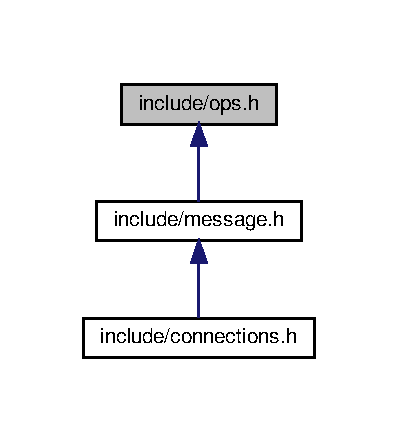
\includegraphics[width=191pt]{ops_8h__dep__incl}
\end{center}
\end{figure}
\subsection*{Enumerations}
\begin{DoxyCompactItemize}
\item 
enum \hyperlink{ops_8h_ac6fa1b34da8872e34c2936391332f44c}{op\+\_\+t} \{ \newline
{\bfseries R\+E\+G\+I\+S\+T\+E\+R\+\_\+\+OP} = 0, 
\hyperlink{ops_8h_ac6fa1b34da8872e34c2936391332f44cab602ddf0795d3c4dc2fd0b4b957ba988}{C\+O\+N\+N\+E\+C\+T\+\_\+\+OP} = 1, 
\hyperlink{ops_8h_ac6fa1b34da8872e34c2936391332f44ca87576ba07c1cfb86b898b212bf927e3b}{P\+O\+S\+T\+T\+X\+T\+\_\+\+OP} = 2, 
\hyperlink{ops_8h_ac6fa1b34da8872e34c2936391332f44cad8bffd524142ec0c418a426344387282}{P\+O\+S\+T\+T\+X\+T\+A\+L\+L\+\_\+\+OP} = 3, 
\newline
\hyperlink{ops_8h_ac6fa1b34da8872e34c2936391332f44caf2b9ae66799c6fdfc938b69f49c9d4e4}{P\+O\+S\+T\+F\+I\+L\+E\+\_\+\+OP} = 4, 
\hyperlink{ops_8h_ac6fa1b34da8872e34c2936391332f44cadb9dcac2886dea585d6851db2a02de4b}{G\+E\+T\+F\+I\+L\+E\+\_\+\+OP} = 5, 
\hyperlink{ops_8h_ac6fa1b34da8872e34c2936391332f44cad40f98fc799cf8b6a8dc25c90464a809}{G\+E\+T\+P\+R\+E\+V\+M\+S\+G\+S\+\_\+\+OP} = 6, 
\hyperlink{ops_8h_ac6fa1b34da8872e34c2936391332f44ca76c5f8cf5dd046fbfe3f0b6a7bce8e90}{U\+S\+R\+L\+I\+S\+T\+\_\+\+OP} = 7, 
\newline
\hyperlink{ops_8h_ac6fa1b34da8872e34c2936391332f44cabc2ab44946aad99a4cda3f0e4abb5b5a}{U\+N\+R\+E\+G\+I\+S\+T\+E\+R\+\_\+\+OP} = 8, 
\hyperlink{ops_8h_ac6fa1b34da8872e34c2936391332f44ca06d81ab3ef58420bbebac2c67dc901e2}{D\+I\+S\+C\+O\+N\+N\+E\+C\+T\+\_\+\+OP} = 9, 
\hyperlink{ops_8h_ac6fa1b34da8872e34c2936391332f44ca30840713ad9050c2d275b31ff8404313}{C\+R\+E\+A\+T\+E\+G\+R\+O\+U\+P\+\_\+\+OP} = 10, 
\hyperlink{ops_8h_ac6fa1b34da8872e34c2936391332f44ca30f53d46265f83a2b0a14d6486a450d5}{A\+D\+D\+G\+R\+O\+U\+P\+\_\+\+OP} = 11, 
\newline
\hyperlink{ops_8h_ac6fa1b34da8872e34c2936391332f44cab9abe0fa4dab90183a19f2f56dfe0d49}{D\+E\+L\+G\+R\+O\+U\+P\+\_\+\+OP} = 12, 
\hyperlink{ops_8h_ac6fa1b34da8872e34c2936391332f44cacc156be86a1cb4bfc0e21d8c72e4971c}{O\+P\+\_\+\+OK} = 20, 
{\bfseries T\+X\+T\+\_\+\+M\+E\+S\+S\+A\+GE} = 21, 
{\bfseries F\+I\+L\+E\+\_\+\+M\+E\+S\+S\+A\+GE} = 22, 
\newline
{\bfseries O\+P\+\_\+\+F\+A\+IL} = 25, 
{\bfseries O\+P\+\_\+\+N\+I\+C\+K\+\_\+\+A\+L\+R\+E\+A\+DY} = 26, 
{\bfseries O\+P\+\_\+\+N\+I\+C\+K\+\_\+\+U\+N\+K\+N\+O\+WN} = 27, 
{\bfseries O\+P\+\_\+\+M\+S\+G\+\_\+\+T\+O\+O\+L\+O\+NG} = 28, 
\newline
{\bfseries O\+P\+\_\+\+N\+O\+\_\+\+S\+U\+C\+H\+\_\+\+F\+I\+LE} = 29, 
{\bfseries O\+P\+\_\+\+E\+ND} = 100
 \}
\end{DoxyCompactItemize}


\subsection{Detailed Description}
Contiene i codici delle operazioni di richiesta e risposta. 



\subsection{Enumeration Type Documentation}
\mbox{\Hypertarget{ops_8h_ac6fa1b34da8872e34c2936391332f44c}\label{ops_8h_ac6fa1b34da8872e34c2936391332f44c}} 
\index{ops.\+h@{ops.\+h}!op\+\_\+t@{op\+\_\+t}}
\index{op\+\_\+t@{op\+\_\+t}!ops.\+h@{ops.\+h}}
\subsubsection{\texorpdfstring{op\+\_\+t}{op\_t}}
{\footnotesize\ttfamily enum \hyperlink{ops_8h_ac6fa1b34da8872e34c2936391332f44c}{op\+\_\+t}}

it describes operations that server manages \begin{DoxyEnumFields}{Enumerator}
\raisebox{\heightof{T}}[0pt][0pt]{\index{C\+O\+N\+N\+E\+C\+T\+\_\+\+OP@{C\+O\+N\+N\+E\+C\+T\+\_\+\+OP}!ops.\+h@{ops.\+h}}\index{ops.\+h@{ops.\+h}!C\+O\+N\+N\+E\+C\+T\+\_\+\+OP@{C\+O\+N\+N\+E\+C\+T\+\_\+\+OP}}}\mbox{\Hypertarget{ops_8h_ac6fa1b34da8872e34c2936391332f44cab602ddf0795d3c4dc2fd0b4b957ba988}\label{ops_8h_ac6fa1b34da8872e34c2936391332f44cab602ddf0795d3c4dc2fd0b4b957ba988}} 
C\+O\+N\+N\+E\+C\+T\+\_\+\+OP&richiesta di registrazione di un ninckname \\
\hline

\raisebox{\heightof{T}}[0pt][0pt]{\index{P\+O\+S\+T\+T\+X\+T\+\_\+\+OP@{P\+O\+S\+T\+T\+X\+T\+\_\+\+OP}!ops.\+h@{ops.\+h}}\index{ops.\+h@{ops.\+h}!P\+O\+S\+T\+T\+X\+T\+\_\+\+OP@{P\+O\+S\+T\+T\+X\+T\+\_\+\+OP}}}\mbox{\Hypertarget{ops_8h_ac6fa1b34da8872e34c2936391332f44ca87576ba07c1cfb86b898b212bf927e3b}\label{ops_8h_ac6fa1b34da8872e34c2936391332f44ca87576ba07c1cfb86b898b212bf927e3b}} 
P\+O\+S\+T\+T\+X\+T\+\_\+\+OP&richiesta di connessione di un client \\
\hline

\raisebox{\heightof{T}}[0pt][0pt]{\index{P\+O\+S\+T\+T\+X\+T\+A\+L\+L\+\_\+\+OP@{P\+O\+S\+T\+T\+X\+T\+A\+L\+L\+\_\+\+OP}!ops.\+h@{ops.\+h}}\index{ops.\+h@{ops.\+h}!P\+O\+S\+T\+T\+X\+T\+A\+L\+L\+\_\+\+OP@{P\+O\+S\+T\+T\+X\+T\+A\+L\+L\+\_\+\+OP}}}\mbox{\Hypertarget{ops_8h_ac6fa1b34da8872e34c2936391332f44cad8bffd524142ec0c418a426344387282}\label{ops_8h_ac6fa1b34da8872e34c2936391332f44cad8bffd524142ec0c418a426344387282}} 
P\+O\+S\+T\+T\+X\+T\+A\+L\+L\+\_\+\+OP&richiesta di invio di un messaggio testuale ad un nickname o groupname \\
\hline

\raisebox{\heightof{T}}[0pt][0pt]{\index{P\+O\+S\+T\+F\+I\+L\+E\+\_\+\+OP@{P\+O\+S\+T\+F\+I\+L\+E\+\_\+\+OP}!ops.\+h@{ops.\+h}}\index{ops.\+h@{ops.\+h}!P\+O\+S\+T\+F\+I\+L\+E\+\_\+\+OP@{P\+O\+S\+T\+F\+I\+L\+E\+\_\+\+OP}}}\mbox{\Hypertarget{ops_8h_ac6fa1b34da8872e34c2936391332f44caf2b9ae66799c6fdfc938b69f49c9d4e4}\label{ops_8h_ac6fa1b34da8872e34c2936391332f44caf2b9ae66799c6fdfc938b69f49c9d4e4}} 
P\+O\+S\+T\+F\+I\+L\+E\+\_\+\+OP&richiesta di invio di un messaggio testuale a tutti gli utenti \\
\hline

\raisebox{\heightof{T}}[0pt][0pt]{\index{G\+E\+T\+F\+I\+L\+E\+\_\+\+OP@{G\+E\+T\+F\+I\+L\+E\+\_\+\+OP}!ops.\+h@{ops.\+h}}\index{ops.\+h@{ops.\+h}!G\+E\+T\+F\+I\+L\+E\+\_\+\+OP@{G\+E\+T\+F\+I\+L\+E\+\_\+\+OP}}}\mbox{\Hypertarget{ops_8h_ac6fa1b34da8872e34c2936391332f44cadb9dcac2886dea585d6851db2a02de4b}\label{ops_8h_ac6fa1b34da8872e34c2936391332f44cadb9dcac2886dea585d6851db2a02de4b}} 
G\+E\+T\+F\+I\+L\+E\+\_\+\+OP&richiesta di invio di un file ad un nickname o groupname \\
\hline

\raisebox{\heightof{T}}[0pt][0pt]{\index{G\+E\+T\+P\+R\+E\+V\+M\+S\+G\+S\+\_\+\+OP@{G\+E\+T\+P\+R\+E\+V\+M\+S\+G\+S\+\_\+\+OP}!ops.\+h@{ops.\+h}}\index{ops.\+h@{ops.\+h}!G\+E\+T\+P\+R\+E\+V\+M\+S\+G\+S\+\_\+\+OP@{G\+E\+T\+P\+R\+E\+V\+M\+S\+G\+S\+\_\+\+OP}}}\mbox{\Hypertarget{ops_8h_ac6fa1b34da8872e34c2936391332f44cad40f98fc799cf8b6a8dc25c90464a809}\label{ops_8h_ac6fa1b34da8872e34c2936391332f44cad40f98fc799cf8b6a8dc25c90464a809}} 
G\+E\+T\+P\+R\+E\+V\+M\+S\+G\+S\+\_\+\+OP&richiesta di recupero di un file \\
\hline

\raisebox{\heightof{T}}[0pt][0pt]{\index{U\+S\+R\+L\+I\+S\+T\+\_\+\+OP@{U\+S\+R\+L\+I\+S\+T\+\_\+\+OP}!ops.\+h@{ops.\+h}}\index{ops.\+h@{ops.\+h}!U\+S\+R\+L\+I\+S\+T\+\_\+\+OP@{U\+S\+R\+L\+I\+S\+T\+\_\+\+OP}}}\mbox{\Hypertarget{ops_8h_ac6fa1b34da8872e34c2936391332f44ca76c5f8cf5dd046fbfe3f0b6a7bce8e90}\label{ops_8h_ac6fa1b34da8872e34c2936391332f44ca76c5f8cf5dd046fbfe3f0b6a7bce8e90}} 
U\+S\+R\+L\+I\+S\+T\+\_\+\+OP&richiesta di recupero della history dei messaggi \\
\hline

\raisebox{\heightof{T}}[0pt][0pt]{\index{U\+N\+R\+E\+G\+I\+S\+T\+E\+R\+\_\+\+OP@{U\+N\+R\+E\+G\+I\+S\+T\+E\+R\+\_\+\+OP}!ops.\+h@{ops.\+h}}\index{ops.\+h@{ops.\+h}!U\+N\+R\+E\+G\+I\+S\+T\+E\+R\+\_\+\+OP@{U\+N\+R\+E\+G\+I\+S\+T\+E\+R\+\_\+\+OP}}}\mbox{\Hypertarget{ops_8h_ac6fa1b34da8872e34c2936391332f44cabc2ab44946aad99a4cda3f0e4abb5b5a}\label{ops_8h_ac6fa1b34da8872e34c2936391332f44cabc2ab44946aad99a4cda3f0e4abb5b5a}} 
U\+N\+R\+E\+G\+I\+S\+T\+E\+R\+\_\+\+OP&richiesta di avere la lista di tutti gli utenti attualmente connessi \\
\hline

\raisebox{\heightof{T}}[0pt][0pt]{\index{D\+I\+S\+C\+O\+N\+N\+E\+C\+T\+\_\+\+OP@{D\+I\+S\+C\+O\+N\+N\+E\+C\+T\+\_\+\+OP}!ops.\+h@{ops.\+h}}\index{ops.\+h@{ops.\+h}!D\+I\+S\+C\+O\+N\+N\+E\+C\+T\+\_\+\+OP@{D\+I\+S\+C\+O\+N\+N\+E\+C\+T\+\_\+\+OP}}}\mbox{\Hypertarget{ops_8h_ac6fa1b34da8872e34c2936391332f44ca06d81ab3ef58420bbebac2c67dc901e2}\label{ops_8h_ac6fa1b34da8872e34c2936391332f44ca06d81ab3ef58420bbebac2c67dc901e2}} 
D\+I\+S\+C\+O\+N\+N\+E\+C\+T\+\_\+\+OP&richiesta di deregistrazione di un nickname o groupname \\
\hline

\raisebox{\heightof{T}}[0pt][0pt]{\index{C\+R\+E\+A\+T\+E\+G\+R\+O\+U\+P\+\_\+\+OP@{C\+R\+E\+A\+T\+E\+G\+R\+O\+U\+P\+\_\+\+OP}!ops.\+h@{ops.\+h}}\index{ops.\+h@{ops.\+h}!C\+R\+E\+A\+T\+E\+G\+R\+O\+U\+P\+\_\+\+OP@{C\+R\+E\+A\+T\+E\+G\+R\+O\+U\+P\+\_\+\+OP}}}\mbox{\Hypertarget{ops_8h_ac6fa1b34da8872e34c2936391332f44ca30840713ad9050c2d275b31ff8404313}\label{ops_8h_ac6fa1b34da8872e34c2936391332f44ca30840713ad9050c2d275b31ff8404313}} 
C\+R\+E\+A\+T\+E\+G\+R\+O\+U\+P\+\_\+\+OP&richiesta di disconnessione \\
\hline

\raisebox{\heightof{T}}[0pt][0pt]{\index{A\+D\+D\+G\+R\+O\+U\+P\+\_\+\+OP@{A\+D\+D\+G\+R\+O\+U\+P\+\_\+\+OP}!ops.\+h@{ops.\+h}}\index{ops.\+h@{ops.\+h}!A\+D\+D\+G\+R\+O\+U\+P\+\_\+\+OP@{A\+D\+D\+G\+R\+O\+U\+P\+\_\+\+OP}}}\mbox{\Hypertarget{ops_8h_ac6fa1b34da8872e34c2936391332f44ca30f53d46265f83a2b0a14d6486a450d5}\label{ops_8h_ac6fa1b34da8872e34c2936391332f44ca30f53d46265f83a2b0a14d6486a450d5}} 
A\+D\+D\+G\+R\+O\+U\+P\+\_\+\+OP&richiesta di creazione di un gruppo \\
\hline

\raisebox{\heightof{T}}[0pt][0pt]{\index{D\+E\+L\+G\+R\+O\+U\+P\+\_\+\+OP@{D\+E\+L\+G\+R\+O\+U\+P\+\_\+\+OP}!ops.\+h@{ops.\+h}}\index{ops.\+h@{ops.\+h}!D\+E\+L\+G\+R\+O\+U\+P\+\_\+\+OP@{D\+E\+L\+G\+R\+O\+U\+P\+\_\+\+OP}}}\mbox{\Hypertarget{ops_8h_ac6fa1b34da8872e34c2936391332f44cab9abe0fa4dab90183a19f2f56dfe0d49}\label{ops_8h_ac6fa1b34da8872e34c2936391332f44cab9abe0fa4dab90183a19f2f56dfe0d49}} 
D\+E\+L\+G\+R\+O\+U\+P\+\_\+\+OP&richiesta di aggiunta ad un gruppo \\
\hline

\raisebox{\heightof{T}}[0pt][0pt]{\index{O\+P\+\_\+\+OK@{O\+P\+\_\+\+OK}!ops.\+h@{ops.\+h}}\index{ops.\+h@{ops.\+h}!O\+P\+\_\+\+OK@{O\+P\+\_\+\+OK}}}\mbox{\Hypertarget{ops_8h_ac6fa1b34da8872e34c2936391332f44cacc156be86a1cb4bfc0e21d8c72e4971c}\label{ops_8h_ac6fa1b34da8872e34c2936391332f44cacc156be86a1cb4bfc0e21d8c72e4971c}} 
O\+P\+\_\+\+OK&richiesta di rimozione da un gruppo \\
\hline

\end{DoxyEnumFields}

\hypertarget{signal__handler_8h}{}\section{include/signal\+\_\+handler.h File Reference}
\label{signal__handler_8h}\index{include/signal\+\_\+handler.\+h@{include/signal\+\_\+handler.\+h}}


it manages all signals triggered by system.  


{\ttfamily \#include $<$stdio.\+h$>$}\newline
{\ttfamily \#include $<$unistd.\+h$>$}\newline
{\ttfamily \#include $<$stdlib.\+h$>$}\newline
{\ttfamily \#include $<$assert.\+h$>$}\newline
{\ttfamily \#include $<$string.\+h$>$}\newline
{\ttfamily \#include $<$signal.\+h$>$}\newline
{\ttfamily \#include $<$pthread.\+h$>$}\newline
{\ttfamily \#include $<$stdbool.\+h$>$}\newline
{\ttfamily \#include $<$errno.\+h$>$}\newline
{\ttfamily \#include \char`\"{}log.\+h\char`\"{}}\newline
Include dependency graph for signal\+\_\+handler.\+h\+:\nopagebreak
\begin{figure}[H]
\begin{center}
\leavevmode
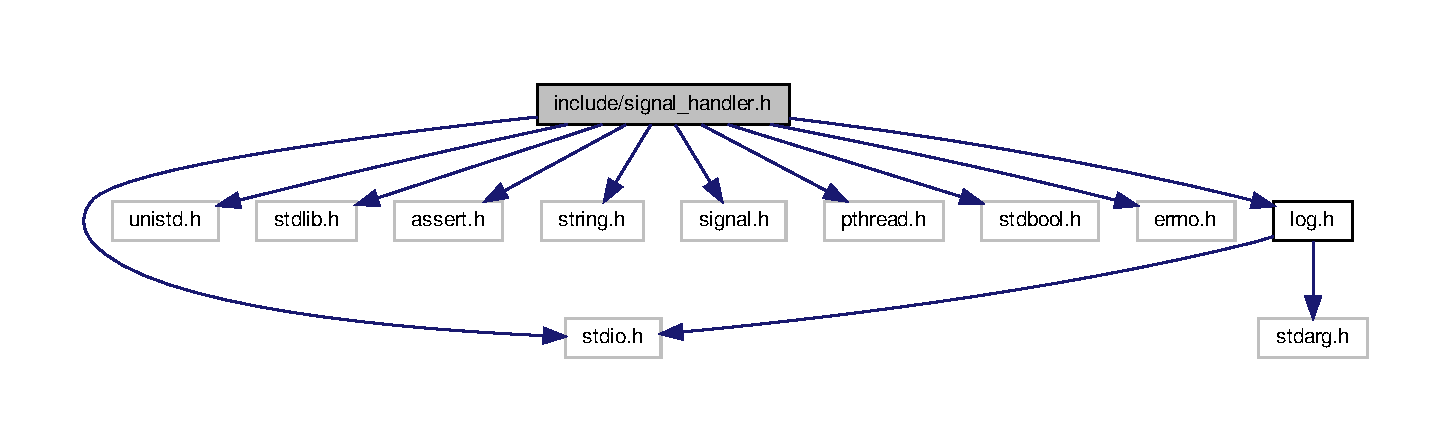
\includegraphics[width=350pt]{signal__handler_8h__incl}
\end{center}
\end{figure}
This graph shows which files directly or indirectly include this file\+:\nopagebreak
\begin{figure}[H]
\begin{center}
\leavevmode
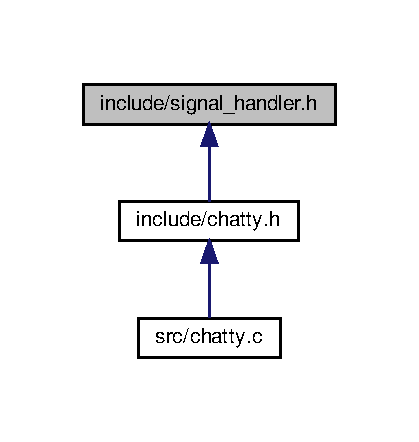
\includegraphics[width=201pt]{signal__handler_8h__dep__incl}
\end{center}
\end{figure}
\subsection*{Macros}
\begin{DoxyCompactItemize}
\item 
\#define \hyperlink{signal__handler_8h_a3024ccd4a9af5109d24e6c57565d74a1}{\+\_\+\+P\+O\+S\+I\+X\+\_\+\+C\+\_\+\+S\+O\+U\+R\+CE}~200809L
\item 
\#define \hyperlink{signal__handler_8h_a5d71cb4e18ade666bf913567d6d4fa97}{S\+I\+G\+\_\+\+H\+A\+N\+D\+L\+\_\+N}~1
\item 
\#define \hyperlink{signal__handler_8h_ad559c55d3a5e4db4aa899b249d996e12}{S\+I\+G\+\_\+\+H\+A\+N\+D\+L\+\_\+\+S\+I\+G\+P\+I\+PE}~0
\item 
\#define \hyperlink{signal__handler_8h_a93840855dbf2a651a4e60c1f4a41ca1a}{S\+I\+G\+\_\+\+H\+A\+N\+D\+L\+\_\+\+S\+I\+G\+T\+E\+RM}~1
\item 
\#define \hyperlink{signal__handler_8h_aebb23c893e4aff2a3dce21bf876ee9b2}{S\+I\+G\+\_\+\+H\+A\+N\+D\+L\+\_\+\+S\+I\+G\+U\+S\+R1}~2
\end{DoxyCompactItemize}
\subsection*{Functions}
\begin{DoxyCompactItemize}
\item 
\mbox{\Hypertarget{signal__handler_8h_aa1d2bef729ebc3056a77a5df3e32eb63}\label{signal__handler_8h_aa1d2bef729ebc3056a77a5df3e32eb63}} 
void \hyperlink{signal__handler_8h_aa1d2bef729ebc3056a77a5df3e32eb63}{signal\+\_\+handler\+\_\+init} ()
\begin{DoxyCompactList}\small\item\em initialize signal handler \end{DoxyCompactList}\item 
bool \hyperlink{signal__handler_8h_a330a89ec83f0052a65a5aeef99f6049a}{signal\+\_\+handler\+\_\+register} ()
\item 
void \hyperlink{signal__handler_8h_a1a393955c54861bb65200b0e8901e0de}{signal\+\_\+handler\+\_\+pipe} ()
\begin{DoxyCompactList}\small\item\em this function manages the S\+I\+G\+P\+I\+PE signal. \end{DoxyCompactList}\item 
void \hyperlink{signal__handler_8h_a27824fe66547c062e9f4f85846ea7843}{signal\+\_\+handler\+\_\+term} ()
\begin{DoxyCompactList}\small\item\em this function manages the operation for stopping server. \end{DoxyCompactList}\item 
void \hyperlink{signal__handler_8h_afc5fae13cf9316bc22850a42e4a9dbc2}{signal\+\_\+handler\+\_\+usr1} ()
\begin{DoxyCompactList}\small\item\em this function manages the statistic printing trigger. \end{DoxyCompactList}\end{DoxyCompactItemize}
\subsection*{Variables}
\begin{DoxyCompactItemize}
\item 
const int \hyperlink{signal__handler_8h_a0934ae8b589ddd7c3ed9580f89d0fb71}{sig\+\_\+handl\+\_\+signals} \mbox{[}$\,$\mbox{]}
\item 
struct sigaction \hyperlink{signal__handler_8h_a28898d23b46e39a72f4e011ad4e221f4}{sig\+\_\+handl\+\_\+acts} \mbox{[}$\,$\mbox{]}
\end{DoxyCompactItemize}


\subsection{Detailed Description}
it manages all signals triggered by system. 

signal management header file. 

\subsection{Macro Definition Documentation}
\mbox{\Hypertarget{signal__handler_8h_a3024ccd4a9af5109d24e6c57565d74a1}\label{signal__handler_8h_a3024ccd4a9af5109d24e6c57565d74a1}} 
\index{signal\+\_\+handler.\+h@{signal\+\_\+handler.\+h}!\+\_\+\+P\+O\+S\+I\+X\+\_\+\+C\+\_\+\+S\+O\+U\+R\+CE@{\+\_\+\+P\+O\+S\+I\+X\+\_\+\+C\+\_\+\+S\+O\+U\+R\+CE}}
\index{\+\_\+\+P\+O\+S\+I\+X\+\_\+\+C\+\_\+\+S\+O\+U\+R\+CE@{\+\_\+\+P\+O\+S\+I\+X\+\_\+\+C\+\_\+\+S\+O\+U\+R\+CE}!signal\+\_\+handler.\+h@{signal\+\_\+handler.\+h}}
\subsubsection{\texorpdfstring{\+\_\+\+P\+O\+S\+I\+X\+\_\+\+C\+\_\+\+S\+O\+U\+R\+CE}{\_POSIX\_C\_SOURCE}}
{\footnotesize\ttfamily \#define \+\_\+\+P\+O\+S\+I\+X\+\_\+\+C\+\_\+\+S\+O\+U\+R\+CE~200809L}

Define Posix Source \mbox{\Hypertarget{signal__handler_8h_a5d71cb4e18ade666bf913567d6d4fa97}\label{signal__handler_8h_a5d71cb4e18ade666bf913567d6d4fa97}} 
\index{signal\+\_\+handler.\+h@{signal\+\_\+handler.\+h}!S\+I\+G\+\_\+\+H\+A\+N\+D\+L\+\_\+N@{S\+I\+G\+\_\+\+H\+A\+N\+D\+L\+\_\+N}}
\index{S\+I\+G\+\_\+\+H\+A\+N\+D\+L\+\_\+N@{S\+I\+G\+\_\+\+H\+A\+N\+D\+L\+\_\+N}!signal\+\_\+handler.\+h@{signal\+\_\+handler.\+h}}
\subsubsection{\texorpdfstring{S\+I\+G\+\_\+\+H\+A\+N\+D\+L\+\_\+N}{SIG\_HANDL\_N}}
{\footnotesize\ttfamily \#define S\+I\+G\+\_\+\+H\+A\+N\+D\+L\+\_\+N~1}

How many signals are registered. \mbox{\Hypertarget{signal__handler_8h_ad559c55d3a5e4db4aa899b249d996e12}\label{signal__handler_8h_ad559c55d3a5e4db4aa899b249d996e12}} 
\index{signal\+\_\+handler.\+h@{signal\+\_\+handler.\+h}!S\+I\+G\+\_\+\+H\+A\+N\+D\+L\+\_\+\+S\+I\+G\+P\+I\+PE@{S\+I\+G\+\_\+\+H\+A\+N\+D\+L\+\_\+\+S\+I\+G\+P\+I\+PE}}
\index{S\+I\+G\+\_\+\+H\+A\+N\+D\+L\+\_\+\+S\+I\+G\+P\+I\+PE@{S\+I\+G\+\_\+\+H\+A\+N\+D\+L\+\_\+\+S\+I\+G\+P\+I\+PE}!signal\+\_\+handler.\+h@{signal\+\_\+handler.\+h}}
\subsubsection{\texorpdfstring{S\+I\+G\+\_\+\+H\+A\+N\+D\+L\+\_\+\+S\+I\+G\+P\+I\+PE}{SIG\_HANDL\_SIGPIPE}}
{\footnotesize\ttfamily \#define S\+I\+G\+\_\+\+H\+A\+N\+D\+L\+\_\+\+S\+I\+G\+P\+I\+PE~0}

S\+I\+G\+P\+I\+PE signal code \mbox{\Hypertarget{signal__handler_8h_a93840855dbf2a651a4e60c1f4a41ca1a}\label{signal__handler_8h_a93840855dbf2a651a4e60c1f4a41ca1a}} 
\index{signal\+\_\+handler.\+h@{signal\+\_\+handler.\+h}!S\+I\+G\+\_\+\+H\+A\+N\+D\+L\+\_\+\+S\+I\+G\+T\+E\+RM@{S\+I\+G\+\_\+\+H\+A\+N\+D\+L\+\_\+\+S\+I\+G\+T\+E\+RM}}
\index{S\+I\+G\+\_\+\+H\+A\+N\+D\+L\+\_\+\+S\+I\+G\+T\+E\+RM@{S\+I\+G\+\_\+\+H\+A\+N\+D\+L\+\_\+\+S\+I\+G\+T\+E\+RM}!signal\+\_\+handler.\+h@{signal\+\_\+handler.\+h}}
\subsubsection{\texorpdfstring{S\+I\+G\+\_\+\+H\+A\+N\+D\+L\+\_\+\+S\+I\+G\+T\+E\+RM}{SIG\_HANDL\_SIGTERM}}
{\footnotesize\ttfamily \#define S\+I\+G\+\_\+\+H\+A\+N\+D\+L\+\_\+\+S\+I\+G\+T\+E\+RM~1}

S\+I\+G\+T\+E\+RM signal code \mbox{\Hypertarget{signal__handler_8h_aebb23c893e4aff2a3dce21bf876ee9b2}\label{signal__handler_8h_aebb23c893e4aff2a3dce21bf876ee9b2}} 
\index{signal\+\_\+handler.\+h@{signal\+\_\+handler.\+h}!S\+I\+G\+\_\+\+H\+A\+N\+D\+L\+\_\+\+S\+I\+G\+U\+S\+R1@{S\+I\+G\+\_\+\+H\+A\+N\+D\+L\+\_\+\+S\+I\+G\+U\+S\+R1}}
\index{S\+I\+G\+\_\+\+H\+A\+N\+D\+L\+\_\+\+S\+I\+G\+U\+S\+R1@{S\+I\+G\+\_\+\+H\+A\+N\+D\+L\+\_\+\+S\+I\+G\+U\+S\+R1}!signal\+\_\+handler.\+h@{signal\+\_\+handler.\+h}}
\subsubsection{\texorpdfstring{S\+I\+G\+\_\+\+H\+A\+N\+D\+L\+\_\+\+S\+I\+G\+U\+S\+R1}{SIG\_HANDL\_SIGUSR1}}
{\footnotesize\ttfamily \#define S\+I\+G\+\_\+\+H\+A\+N\+D\+L\+\_\+\+S\+I\+G\+U\+S\+R1~2}

S\+I\+G\+U\+S\+R1 signal code 

\subsection{Function Documentation}
\mbox{\Hypertarget{signal__handler_8h_a1a393955c54861bb65200b0e8901e0de}\label{signal__handler_8h_a1a393955c54861bb65200b0e8901e0de}} 
\index{signal\+\_\+handler.\+h@{signal\+\_\+handler.\+h}!signal\+\_\+handler\+\_\+pipe@{signal\+\_\+handler\+\_\+pipe}}
\index{signal\+\_\+handler\+\_\+pipe@{signal\+\_\+handler\+\_\+pipe}!signal\+\_\+handler.\+h@{signal\+\_\+handler.\+h}}
\subsubsection{\texorpdfstring{signal\+\_\+handler\+\_\+pipe()}{signal\_handler\_pipe()}}
{\footnotesize\ttfamily void signal\+\_\+handler\+\_\+pipe (\begin{DoxyParamCaption}{ }\end{DoxyParamCaption})}



this function manages the S\+I\+G\+P\+I\+PE signal. 

Handler for S\+I\+G\+P\+I\+PE \mbox{\Hypertarget{signal__handler_8h_a330a89ec83f0052a65a5aeef99f6049a}\label{signal__handler_8h_a330a89ec83f0052a65a5aeef99f6049a}} 
\index{signal\+\_\+handler.\+h@{signal\+\_\+handler.\+h}!signal\+\_\+handler\+\_\+register@{signal\+\_\+handler\+\_\+register}}
\index{signal\+\_\+handler\+\_\+register@{signal\+\_\+handler\+\_\+register}!signal\+\_\+handler.\+h@{signal\+\_\+handler.\+h}}
\subsubsection{\texorpdfstring{signal\+\_\+handler\+\_\+register()}{signal\_handler\_register()}}
{\footnotesize\ttfamily bool signal\+\_\+handler\+\_\+register (\begin{DoxyParamCaption}{ }\end{DoxyParamCaption})}

This function registers all handlers for program. If any errors occurs function will print it. \begin{DoxyReturn}{Returns}
false in case of error 
\end{DoxyReturn}
\mbox{\Hypertarget{signal__handler_8h_a27824fe66547c062e9f4f85846ea7843}\label{signal__handler_8h_a27824fe66547c062e9f4f85846ea7843}} 
\index{signal\+\_\+handler.\+h@{signal\+\_\+handler.\+h}!signal\+\_\+handler\+\_\+term@{signal\+\_\+handler\+\_\+term}}
\index{signal\+\_\+handler\+\_\+term@{signal\+\_\+handler\+\_\+term}!signal\+\_\+handler.\+h@{signal\+\_\+handler.\+h}}
\subsubsection{\texorpdfstring{signal\+\_\+handler\+\_\+term()}{signal\_handler\_term()}}
{\footnotesize\ttfamily void signal\+\_\+handler\+\_\+term (\begin{DoxyParamCaption}{ }\end{DoxyParamCaption})}



this function manages the operation for stopping server. 

Handler for S\+I\+G\+T\+E\+RM. \mbox{\Hypertarget{signal__handler_8h_afc5fae13cf9316bc22850a42e4a9dbc2}\label{signal__handler_8h_afc5fae13cf9316bc22850a42e4a9dbc2}} 
\index{signal\+\_\+handler.\+h@{signal\+\_\+handler.\+h}!signal\+\_\+handler\+\_\+usr1@{signal\+\_\+handler\+\_\+usr1}}
\index{signal\+\_\+handler\+\_\+usr1@{signal\+\_\+handler\+\_\+usr1}!signal\+\_\+handler.\+h@{signal\+\_\+handler.\+h}}
\subsubsection{\texorpdfstring{signal\+\_\+handler\+\_\+usr1()}{signal\_handler\_usr1()}}
{\footnotesize\ttfamily void signal\+\_\+handler\+\_\+usr1 (\begin{DoxyParamCaption}{ }\end{DoxyParamCaption})}



this function manages the statistic printing trigger. 

Handler for S\+I\+G\+U\+S\+R1. 

\subsection{Variable Documentation}
\mbox{\Hypertarget{signal__handler_8h_a28898d23b46e39a72f4e011ad4e221f4}\label{signal__handler_8h_a28898d23b46e39a72f4e011ad4e221f4}} 
\index{signal\+\_\+handler.\+h@{signal\+\_\+handler.\+h}!sig\+\_\+handl\+\_\+acts@{sig\+\_\+handl\+\_\+acts}}
\index{sig\+\_\+handl\+\_\+acts@{sig\+\_\+handl\+\_\+acts}!signal\+\_\+handler.\+h@{signal\+\_\+handler.\+h}}
\subsubsection{\texorpdfstring{sig\+\_\+handl\+\_\+acts}{sig\_handl\_acts}}
{\footnotesize\ttfamily struct sigaction sig\+\_\+handl\+\_\+acts\mbox{[}$\,$\mbox{]}}

Actions to perform when signal is triggered. \mbox{\Hypertarget{signal__handler_8h_a0934ae8b589ddd7c3ed9580f89d0fb71}\label{signal__handler_8h_a0934ae8b589ddd7c3ed9580f89d0fb71}} 
\index{signal\+\_\+handler.\+h@{signal\+\_\+handler.\+h}!sig\+\_\+handl\+\_\+signals@{sig\+\_\+handl\+\_\+signals}}
\index{sig\+\_\+handl\+\_\+signals@{sig\+\_\+handl\+\_\+signals}!signal\+\_\+handler.\+h@{signal\+\_\+handler.\+h}}
\subsubsection{\texorpdfstring{sig\+\_\+handl\+\_\+signals}{sig\_handl\_signals}}
{\footnotesize\ttfamily const int sig\+\_\+handl\+\_\+signals\mbox{[}$\,$\mbox{]}}

Registered signal to register to system 
\hypertarget{chatty_8c}{}\section{src/chatty.c File Reference}
\label{chatty_8c}\index{src/chatty.\+c@{src/chatty.\+c}}


File principale del server chatterbox.  


{\ttfamily \#include $<$stdio.\+h$>$}\newline
{\ttfamily \#include $<$unistd.\+h$>$}\newline
{\ttfamily \#include $<$stdlib.\+h$>$}\newline
{\ttfamily \#include $<$assert.\+h$>$}\newline
{\ttfamily \#include $<$string.\+h$>$}\newline
{\ttfamily \#include $<$signal.\+h$>$}\newline
{\ttfamily \#include $<$pthread.\+h$>$}\newline
{\ttfamily \#include \char`\"{}chatty.\+h\char`\"{}}\newline
Include dependency graph for chatty.\+c\+:\nopagebreak
\begin{figure}[H]
\begin{center}
\leavevmode
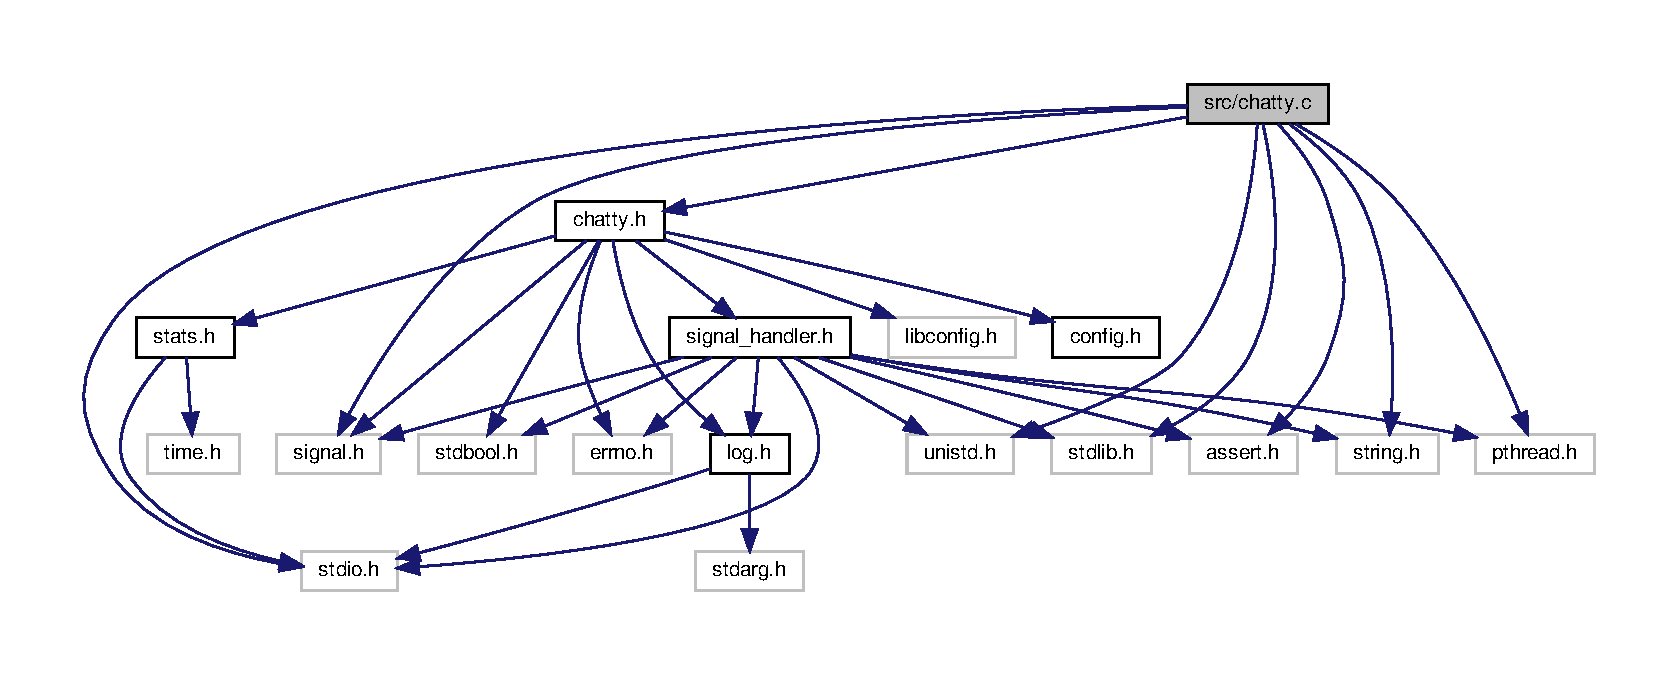
\includegraphics[width=350pt]{chatty_8c__incl}
\end{center}
\end{figure}
\subsection*{Macros}
\begin{DoxyCompactItemize}
\item 
\#define \hyperlink{chatty_8c_a3024ccd4a9af5109d24e6c57565d74a1}{\+\_\+\+P\+O\+S\+I\+X\+\_\+\+C\+\_\+\+S\+O\+U\+R\+CE}~200809L
\end{DoxyCompactItemize}
\subsection*{Functions}
\begin{DoxyCompactItemize}
\item 
int \hyperlink{chatty_8c_a0ddf1224851353fc92bfbff6f499fa97}{main} (int argc, char $\ast$argv\mbox{[}$\,$\mbox{]})
\item 
bool \hyperlink{chatty_8c_aad12432f8ae837b800280246037a3c1c}{check\+\_\+arguments} (int argc, char $\ast$argv\mbox{[}$\,$\mbox{]})
\item 
bool \hyperlink{chatty_8c_a9d083242d81f6a5b934b560402526368}{parse\+\_\+config} (char $\ast$conf\+\_\+file\+\_\+path)
\begin{DoxyCompactList}\small\item\em This function load into memory the file passed as configuration file. If any problem occurs during loading it returns false. \end{DoxyCompactList}\item 
\mbox{\Hypertarget{chatty_8c_af6fb578a8004391d404dce76d9ee0351}\label{chatty_8c_af6fb578a8004391d404dce76d9ee0351}} 
void \hyperlink{chatty_8c_af6fb578a8004391d404dce76d9ee0351}{clean\+\_\+workspace} ()
\begin{DoxyCompactList}\small\item\em clean workspace from any leaks. \end{DoxyCompactList}\end{DoxyCompactItemize}
\subsection*{Variables}
\begin{DoxyCompactItemize}
\item 
struct \hyperlink{structstatistics}{statistics} \hyperlink{chatty_8c_a9e4166354e886d074465ab1bb87ca0e2}{chatty\+Stats} = \{ 0, 0, 0, 0, 0, 0, 0 \}
\end{DoxyCompactItemize}


\subsection{Detailed Description}
File principale del server chatterbox. 



\subsection{Macro Definition Documentation}
\mbox{\Hypertarget{chatty_8c_a3024ccd4a9af5109d24e6c57565d74a1}\label{chatty_8c_a3024ccd4a9af5109d24e6c57565d74a1}} 
\index{chatty.\+c@{chatty.\+c}!\+\_\+\+P\+O\+S\+I\+X\+\_\+\+C\+\_\+\+S\+O\+U\+R\+CE@{\+\_\+\+P\+O\+S\+I\+X\+\_\+\+C\+\_\+\+S\+O\+U\+R\+CE}}
\index{\+\_\+\+P\+O\+S\+I\+X\+\_\+\+C\+\_\+\+S\+O\+U\+R\+CE@{\+\_\+\+P\+O\+S\+I\+X\+\_\+\+C\+\_\+\+S\+O\+U\+R\+CE}!chatty.\+c@{chatty.\+c}}
\subsubsection{\texorpdfstring{\+\_\+\+P\+O\+S\+I\+X\+\_\+\+C\+\_\+\+S\+O\+U\+R\+CE}{\_POSIX\_C\_SOURCE}}
{\footnotesize\ttfamily \#define \+\_\+\+P\+O\+S\+I\+X\+\_\+\+C\+\_\+\+S\+O\+U\+R\+CE~200809L}

C P\+O\+S\+IX source definition. 

\subsection{Function Documentation}
\mbox{\Hypertarget{chatty_8c_aad12432f8ae837b800280246037a3c1c}\label{chatty_8c_aad12432f8ae837b800280246037a3c1c}} 
\index{chatty.\+c@{chatty.\+c}!check\+\_\+arguments@{check\+\_\+arguments}}
\index{check\+\_\+arguments@{check\+\_\+arguments}!chatty.\+c@{chatty.\+c}}
\subsubsection{\texorpdfstring{check\+\_\+arguments()}{check\_arguments()}}
{\footnotesize\ttfamily bool check\+\_\+arguments (\begin{DoxyParamCaption}\item[{int}]{argc,  }\item[{char $\ast$}]{argv\mbox{[}$\,$\mbox{]} }\end{DoxyParamCaption})}

This function checks if argument passed by system are valid or not.


\begin{DoxyParams}{Parameters}
{\em argc} & system argument count \\
\hline
{\em argv} & system argument \\
\hline
\end{DoxyParams}
\begin{DoxyReturn}{Returns}
true if arguments are valid, false otherwise 
\end{DoxyReturn}
\mbox{\Hypertarget{chatty_8c_a0ddf1224851353fc92bfbff6f499fa97}\label{chatty_8c_a0ddf1224851353fc92bfbff6f499fa97}} 
\index{chatty.\+c@{chatty.\+c}!main@{main}}
\index{main@{main}!chatty.\+c@{chatty.\+c}}
\subsubsection{\texorpdfstring{main()}{main()}}
{\footnotesize\ttfamily int main (\begin{DoxyParamCaption}\item[{int}]{argc,  }\item[{char $\ast$}]{argv\mbox{[}$\,$\mbox{]} }\end{DoxyParamCaption})}

Main function that is called from system. 
\begin{DoxyParams}{Parameters}
{\em argc} & argument count \\
\hline
{\em argv} & array of string that contains arguments \\
\hline
\end{DoxyParams}
\begin{DoxyReturn}{Returns}
program exit code. 
\end{DoxyReturn}
\mbox{\Hypertarget{chatty_8c_a9d083242d81f6a5b934b560402526368}\label{chatty_8c_a9d083242d81f6a5b934b560402526368}} 
\index{chatty.\+c@{chatty.\+c}!parse\+\_\+config@{parse\+\_\+config}}
\index{parse\+\_\+config@{parse\+\_\+config}!chatty.\+c@{chatty.\+c}}
\subsubsection{\texorpdfstring{parse\+\_\+config()}{parse\_config()}}
{\footnotesize\ttfamily bool parse\+\_\+config (\begin{DoxyParamCaption}\item[{char $\ast$}]{conf\+\_\+file\+\_\+path }\end{DoxyParamCaption})}



This function load into memory the file passed as configuration file. If any problem occurs during loading it returns false. 


\begin{DoxyParams}{Parameters}
{\em conf\+\_\+file\+\_\+path} & string that represents the path of config file. \\
\hline
\end{DoxyParams}


\subsection{Variable Documentation}
\mbox{\Hypertarget{chatty_8c_a9e4166354e886d074465ab1bb87ca0e2}\label{chatty_8c_a9e4166354e886d074465ab1bb87ca0e2}} 
\index{chatty.\+c@{chatty.\+c}!chatty\+Stats@{chatty\+Stats}}
\index{chatty\+Stats@{chatty\+Stats}!chatty.\+c@{chatty.\+c}}
\subsubsection{\texorpdfstring{chatty\+Stats}{chattyStats}}
{\footnotesize\ttfamily struct \hyperlink{structstatistics}{statistics} chatty\+Stats = \{ 0, 0, 0, 0, 0, 0, 0 \}}

Variable to register statistics. 
%--- End generated contents ---

% Index
\backmatter
\newpage
\phantomsection
\clearemptydoublepage
\addcontentsline{toc}{chapter}{Index}
\printindex

\end{document}
